\documentclass[a4paper, 10pt]{article}
\usepackage[left=2cm, right =2cm, top=2cm, bottom=3cm]{geometry}
% Useful packages
\usepackage{amsmath,physics, amssymb}
\usepackage{graphicx}
\usepackage[colorlinks=true, allcolors=blue]{hyperref}
\usepackage{color}
\newcommand{\blue}[1]{\textcolor{blue}{#1}}
\newcommand{\red}[1]{\textcolor{red}{#1}}
\usepackage{soul, ulem, todonotes}
%\usepackage{mathptmx}

\usepackage[capitalise]{cleveref}
%\usepackage[backend=bibtex, citestyle=numeric-comp, sorting=none, url =false]{biblatex}
\usepackage[backend=biber, style=numeric]{biblatex}
\addbibresource[]{discussion.bib}  
% Include bibliography from discussion.bib
% The bibliography will be printed at the end using \printbibliography{}
\setcounter{tocdepth}{2}

% Sans modern font
%\usepackage{sansmath}
%\renewcommand{\familydefault}{\sfdefault}
%\sansmath

\title{Impurity induced flat-band discrete time crystal}
\usepackage{authblk}
\author[1]{Mahbub Rahaman}
\author[1]{Sayan Choudhury}
\affil[1]{\small Harish-Chandra Research Institute, HBNI, Chhatnag Road, Jhunsi, Praygraj, UP - 211019, India}
\date{}
\begin{document}
\maketitle
%\tableofcontents
%\newpage

\section{The Model and Dynamics}
We investigate a flat-band protocol arising from a carefully engineered two-frequency periodic drive. The time-dependent Hamiltonian of the system is defined as
\begin{align}
    \hat{\mathcal{H}}_{\text{total}}(t) &=  \hat{\mathcal{H}}_0(t) + \hat{\mathcal{H}}_1(t)  + \hat{\mathcal{H}}_2(t), \\
    \hat{\mathcal{H}}_0(t) &= J(t)\sum_{j} \hat{\sigma}_j^z \hat{\sigma}_{j+1}^z, \quad J(t) = J\, \mathrm{sgn}[\cos(\omega t)], \\
    \hat{\mathcal{H}}_1(t) &= g(t)\sum_{j}\hat{\sigma}_j^x, \quad g(t) = g\, \mathrm{sgn}[\cos(2 \omega t)], \\
    \hat{\mathcal{H}}_2(t) &=
    \begin{cases}
        0, & 0 < t \leq \frac{T}{2}, \\
        \lambda_s \sum_{j}\hat{\sigma}_j^x, & \frac{T}{2} < t \leq T,
    \end{cases}
\end{align}
where $\hat{\sigma}_j^{x,y,z}$ are the Pauli matrices at site $j$, $J$ denotes the Ising interaction strength, $g$ is the transverse field amplitude, and $\lambda_s$ is the amplitude of the secondary drive, chosen such that $\lambda_s \frac{T}{2} = \frac{\pi}{2}$. The primary drive has period $T = 2\pi/\omega$. The system is subjected to two square pulse drives at frequencies $\omega$ and $2\omega$. The first term, $\hat{\mathcal{H}}_0(t)$, represents a periodically modulated Ising interaction, while the second term, $\hat{\mathcal{H}}_1(t)$, corresponds to a periodically driven transverse field. Together, these drives establish the flat-band protocol, resulting in completely localized states (CLS). The third term, $\hat{\mathcal{H}}_2(t)$, implements a global spin-flip operation during the second half of each period, inducing a period-doubled response and ultimately leading to a discrete time crystal (DTC) phase.

The Floquet Hamiltonian, $\hat{\mathcal{H}}_F$, is defined via the relation $\hat{U}(T,0) = e^{-i \hat{\mathcal{H}}_F T}$, where $\hat{U}(T,0)$ is the time-evolution operator over one period $T$. Explicitly,
\begin{align}
    \hat{\mathcal{H}}_F = \frac{i}{T} \ln[\hat{U}(T,0)].
\end{align}

Employing the Suzuki-Trotter decomposition and Zassenhaus’ formula, the propagator can be expressed as

\begin{align}
    \hat{U}(T,0) =& \exp\left(-i \lambda_s \frac{T}{2} \sum_{j}\hat{\sigma}_j^x\right)
    \exp\left(i g \frac{T}{4} \sum_{j}\hat{\sigma}_j^x\right)
    \exp\left(-i g \frac{T}{4} \sum_{j}\hat{\sigma}_j^x\right)\exp\left(i J \frac{T}{2} \sum_{j} \hat{\sigma}_j^z \hat{\sigma}_{j+1}^z\right)\nonumber\\
    &\hspace{4cm}\exp\left(i g \frac{T}{4} \sum_{j}\hat{\sigma}_j^x\right)\exp\left(-i g \frac{T}{4} \sum_{j}\hat{\sigma}_j^x\right)\exp\left(-i J \frac{T}{2} \sum_{j} \hat{\sigma}_j^z \hat{\sigma}_{j+1}^z\right).
\end{align}
The Floquet Hamiltonian can be computed numerically by evaluating the logarithm of the propagator, and its quasienergy spectrum is obtained by diagonalizing $\hat{\mathcal{H}}_F$.

\subsection{Flat-Band Protocol and Emergent CLS}
In the absence of the spin-flip operation $\hat{\mathcal{H}}_2(t)$, the system is governed by a reduced Hamiltonian expected to exhibit a flat band in its quasienergy spectrum:
\begin{align}
    \hat{\mathcal{H}}_{\text{eff}}(t) = \hat{\mathcal{H}}_0(t) + \hat{\mathcal{H}}_1(t).
\end{align}
The corresponding Floquet Hamiltonian is defined by $\hat{U}_{\text{eff}}(T,0) = e^{-i \hat{\mathcal{H}}_{\text{eff},F} T}$, with the propagator given by
\begin{align}
    \hat{U}_{\text{eff}}(T,0) =& 
    \exp\left(i g \frac{T}{4} \sum_{j}\hat{\sigma}_j^x\right)
    \exp\left(-i g \frac{T}{4} \sum_{j}\hat{\sigma}_j^x\right)\exp\left(i J \frac{T}{2} \sum_{j} \hat{\sigma}_j^z \hat{\sigma}_{j+1}^z\right)\nonumber\\
    &\hspace{4cm}\exp\left(i g \frac{T}{4} \sum_{j}\hat{\sigma}_j^x\right)\exp\left(-i g \frac{T}{4} \sum_{j}\hat{\sigma}_j^x\right)\exp\left(-i J \frac{T}{2} \sum_{j} \hat{\sigma}_j^z \hat{\sigma}_{j+1}^z\right).
\end{align}
Neglecting higher-order commutators via the Suzuki-Trotter decomposition and Zassenhaus’ formula, the propagator simplifies to
\begin{align}
    \hat{U}_{\text{eff}}(T,0) =& 
        \exp\left(i g \frac{T}{4} \sum_{j}\hat{\sigma}_j^x\right)
        \exp\left(-i g \frac{T}{4} \sum_{j}\hat{\sigma}_j^x\right)\exp\left(i J \frac{T}{2} \sum_{j} \hat{\sigma}_j^z \hat{\sigma}_{j+1}^z\right)\nonumber\\
        &\hspace{4cm}\exp\left(i g \frac{T}{4} \sum_{j}\hat{\sigma}_j^x\right)\exp\left(-i g \frac{T}{4} \sum_{j}\hat{\sigma}_j^x\right)\exp\left(-i J \frac{T}{2} \sum_{j} \hat{\sigma}_j^z \hat{\sigma}_{j+1}^z\right)\nonumber\\
        =& \mathbb{I}.
\end{align}
Thus, $\hat{\mathcal{H}}_{\text{eff},F} = 0$, indicating a completely flat quasienergy spectrum. This analytical result is confirmed by numerical simulations, as shown in \cref{fig:drive}.

\begin{figure}[h!]
    \centering
    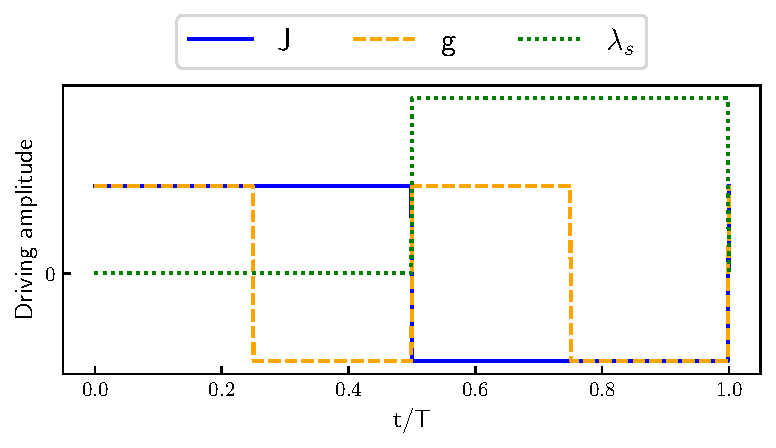
\includegraphics[width=0.45\textwidth]{figs/drive.pdf}
    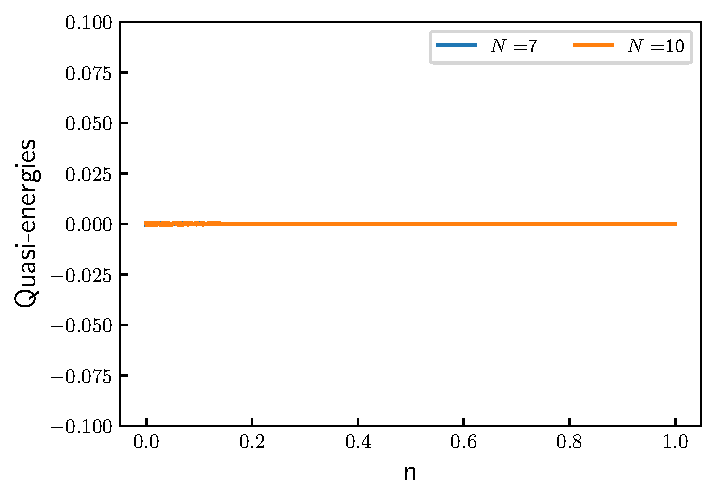
\includegraphics[width=0.4\textwidth]{figs/pure_flatband.pdf}
    \caption{Schematic illustration of the two-frequency drive protocol. The first drive, $\hat{\mathcal{H}}_0(t)$, is a square pulse with period $T$, while the second drive, $\hat{\mathcal{H}}_1(t)$, is a square pulse with period $T/2$. The third component, $\hat{\mathcal{H}}_2(t)$, implements a spin-flip operation during the latter half of each period. The right panel shows the quasienergy spectrum of the effective Floquet Hamiltonian (flat-band only), $\hat{\mathcal{H}}_{\text{eff},F}$, which exhibits a perfectly flat band structure. Parameters: $J=0.18$, $g=J/2$, system sizes $L=7, 10$.}
    \label{fig:drive}
\end{figure}

\subsection{Impurity in the Flat-Band Protocol and Emergent DTC}
Introducing the spin-flip operation $\hat{\mathcal{H}}_2(t)$ acts as an impurity within the flat-band protocol. This term flips all spins during the second half of each period, resulting in a period-doubled response in the system's dynamics. The full Floquet Hamiltonian, $\hat{\mathcal{H}}_F$, incorporates all three components of the time-dependent Hamiltonian. The spin-flip operation disrupts the perfect flatness of the quasienergy spectrum, yielding a non-trivial band structure.

We numerically analyze the magnetization dynamics by initializing the system in a fully polarized state, $\ket{\psi(0)} = \ket{\uparrow \uparrow \uparrow \ldots \uparrow}$. The time evolution of the magnetization at site $j$ is given by
\begin{align}
    m_j(t) = \bra{\psi(t)} \hat{\sigma}_j^z \ket{\psi(t)},
\end{align}
where $\ket{\psi(t)} = \hat{U}(t,0) \ket{\psi(0)}$. The magnetization exhibits oscillations with period $2T$, signifying the emergence of a discrete time crystal phase. However, the stability of this DTC phase is compromised by the impurity term, leading to a gradual decay of the oscillations, as illustrated in Fig.~\ref{figs:impure_flatband_dtc}.
\begin{figure}[h!]
    \centering
    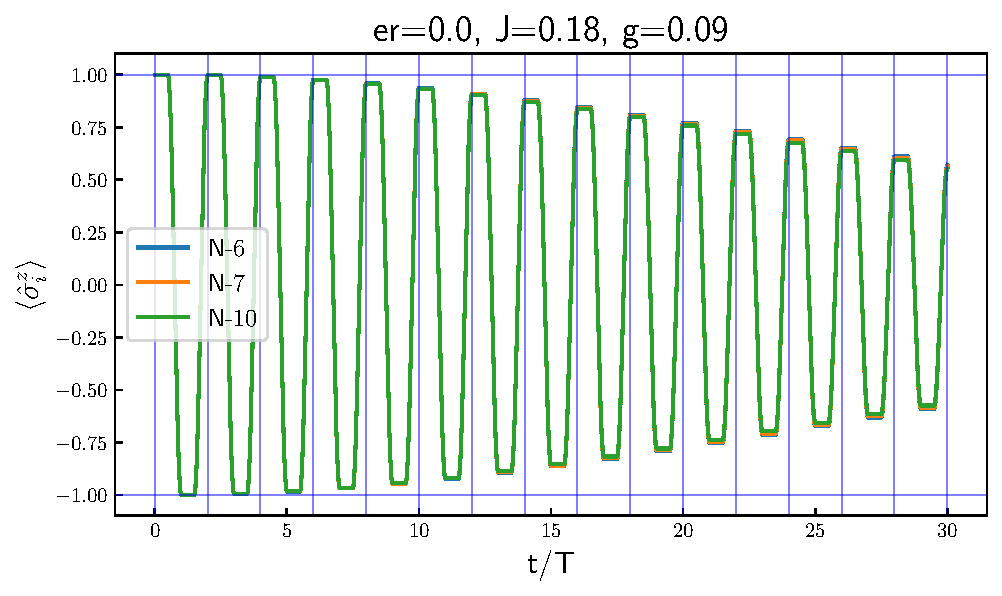
\includegraphics[width=0.45\textwidth]{figs/mag_er0.0_J0.18_g0.09.pdf}
    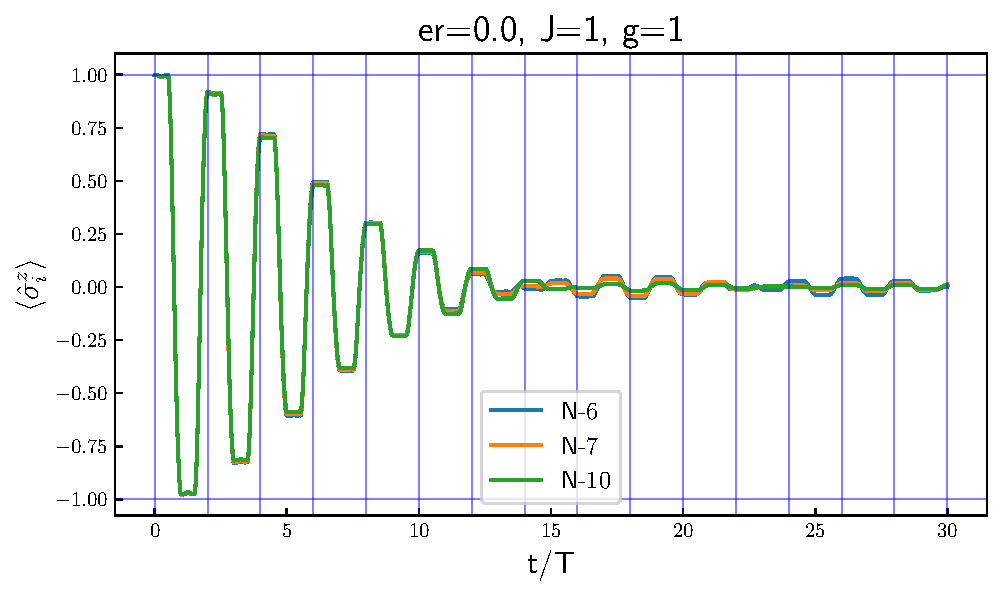
\includegraphics[width=0.45\textwidth]{figs/mag_er0.0_J1_g1.pdf}
    \caption{Time evolution of the magnetization for a system initialized in the fully polarized state, $\ket{\psi(0)} = \ket{\uparrow \uparrow \uparrow \ldots \uparrow}$. Left: Magnetization dynamics for moderate interaction strength ($J=0.18$, $g=J/2$), showing gradual decay of period-doubled oscillations due to the impurity term. Right: Stronger interactions ($J=1$, $g=1$) result in more rapid decay and faster loss of DTC order. In both cases, the impurity-induced spin-flip operation breaks the flatness of the quasienergy spectrum, leading to relaxation and dephasing.}
    \label{figs:impure_flatband_dtc}
\end{figure}

This decay arises from the non-zero bandwidth introduced by the spin-flip operation, which facilitates dephasing and relaxation processes. The quasienergy spectrum of the full Floquet Hamiltonian, $\hat{\mathcal{H}}_F$, is depicted in Fig.~\ref{figs:impure_flatband_qe}, highlighting the deviation from the flat-band structure.
\begin{figure}[h!]
    \centering
    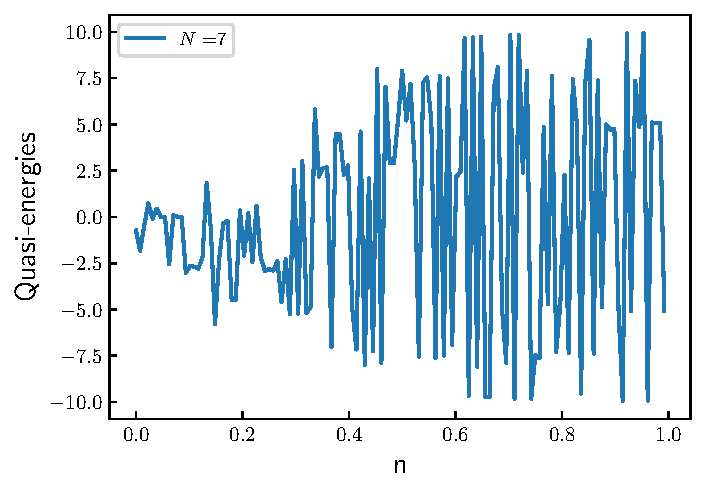
\includegraphics[width=0.45\textwidth]{figs/impure_flatband_qe.pdf}
    \caption{Quasienergy spectrum of the full Floquet Hamiltonian, $\hat{\mathcal{H}}_F$, including the impurity term $\hat{\mathcal{H}}_2(t)$. Parameters: $J=0.18$, $g=J/2$, system size $L=7$, drive frequency $\omega=20$. The impurity induces a non-zero bandwidth in the range $\in[-\omega/2 , \omega/2]$, breaking the perfect flatness of the quasienergy spectrum.}
    \label{figs:impure_flatband_qe}
\end{figure}

\subsection{Flatband DTC}
The flat-band protocol, combined with the impurity term $\hat{\mathcal{H}}_2(t)$, manifests a discrete time crystal (DTC) phase with period-doubled magnetization oscillations. The spin flip operation disrupts the perfect flatness of the quasienergy spectrum, leading to a non-zero bandwidth that causes dephasing and relaxation. The stability of the DTC phase is influenced by the interplay between the transverse field and Ising interaction strengths. To enhance the robustness of the DTC phase, we explore alternative spin-spin Ising interactions and transverse fields, resulting in a modified Hamiltonian:


\begin{align}
    \hat{\mathcal{H}}_{\text{total}}(t) &=  \hat{\mathcal{H}}_0(t) + \hat{\mathcal{H}}_1(t)  + \hat{\mathcal{H}}_2(t), \\
    \hat{\mathcal{H}}_0(t) &= J(t)\sum_{j} \hat{\sigma}_j^x \hat{\sigma}_{j+1}^x, \quad J(t) = J\, \mathrm{sgn}[\cos(\omega t)], \\
    \hat{\mathcal{H}}_1(t) &= g(t)\sum_{j}\hat{\sigma}_j^z, \quad g(t) = g\, \mathrm{sgn}[\cos(2 \omega t)], \\
    \hat{\mathcal{H}}_2(t) &=
    \begin{cases}
        0, & 0 < t \leq \frac{T}{2}, \\
        \lambda_s (1- \epsilon)\sum_{j}\hat{\sigma}_j^x, & \frac{T}{2} < t \leq T,
    \end{cases}
\end{align}
where the spin-flip operation is now implemented along the $x$-direction. This modification aims to avoid additional contribution to the spin rotation errors and enhance the DTC phase's stability. 

We have numerically calculated the magnetization dynamics for this modified Hamiltonian, starting from the fully polarized state $\ket{\psi(0)} = \ket{\uparrow \uparrow \uparrow \ldots \uparrow}$ and at perfect protocol, ie. zero rotational error $\epsilon = 0$. The results, shown in Fig.~\ref{figs:clean_flatband_dtc}, demonstrate more robust period-doubled oscillations with approximately zero melting rate. This indicates that the choice of interaction and transverse field directions plays a crucial role in stabilizing the DTC phase against dephasing and relaxation processes.

\begin{figure}[h!]
    \centering
    
\includegraphics[height=5cm]{figs/DTC_mag_inset_er=0.0_J=0.18_g=0.09.pdf}
    \caption{}
    \label{figs:clean_flatband_dtc}
\end{figure}

However, introducing a small rotational error ($\epsilon = 0.03$) in the spin-flip operation leads to a gradual decay of the DTC phase, as depicted in Fig.~\ref{figs:clean_flatband_dtc_er}. This suggests that while the modified Hamiltonian enhances the DTC phase's stability, it remains sensitive to imperfections in the driving protocol.

\begin{figure}[h!]
    \centering
    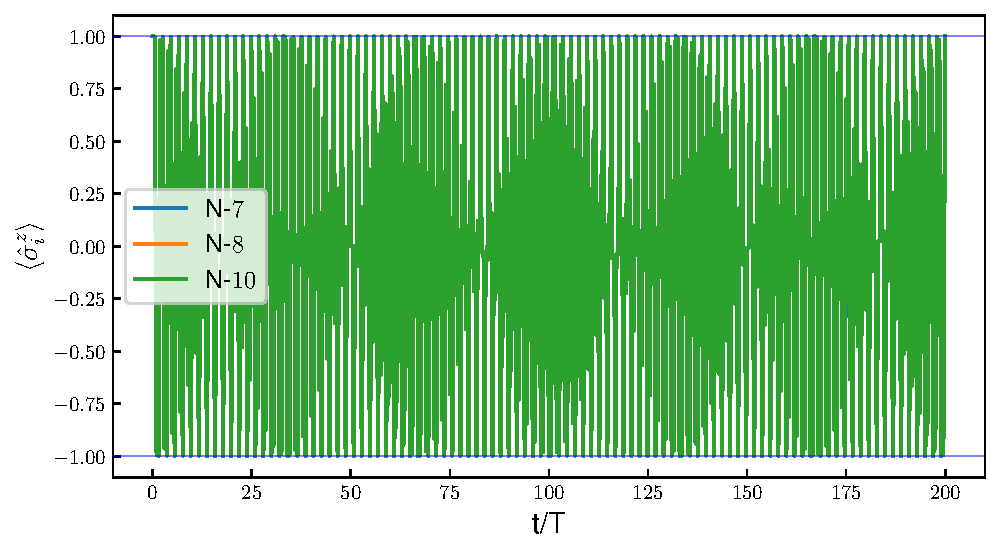
\includegraphics[width=0.45\textwidth]{figs/DTC_mag_inset_er=0.03_J=0.18_g=0.09.pdf}
    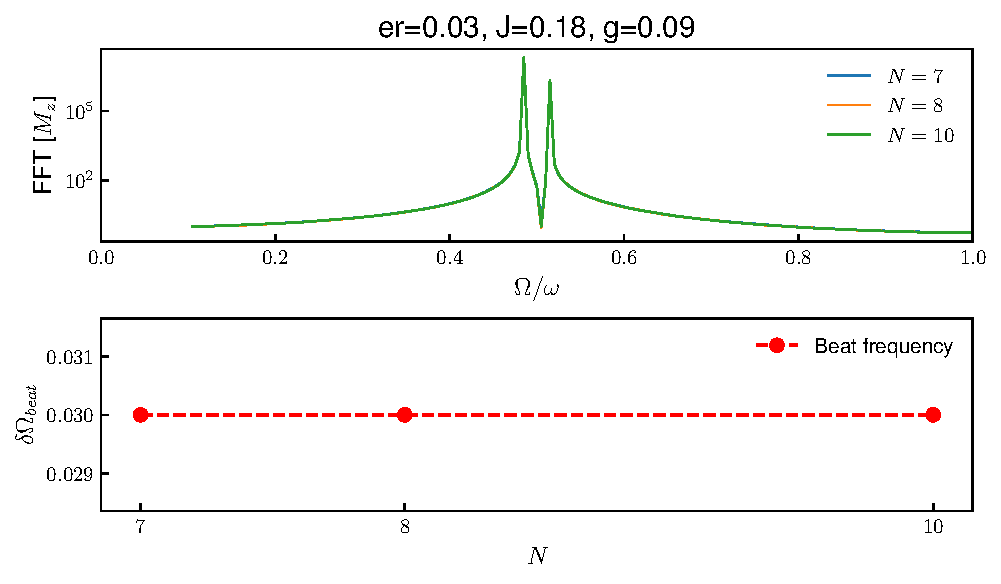
\includegraphics[width=0.45\textwidth]{figs/DTC_mag_fft_inset_er=0.03_J=0.18_g=0.09.pdf}\\
    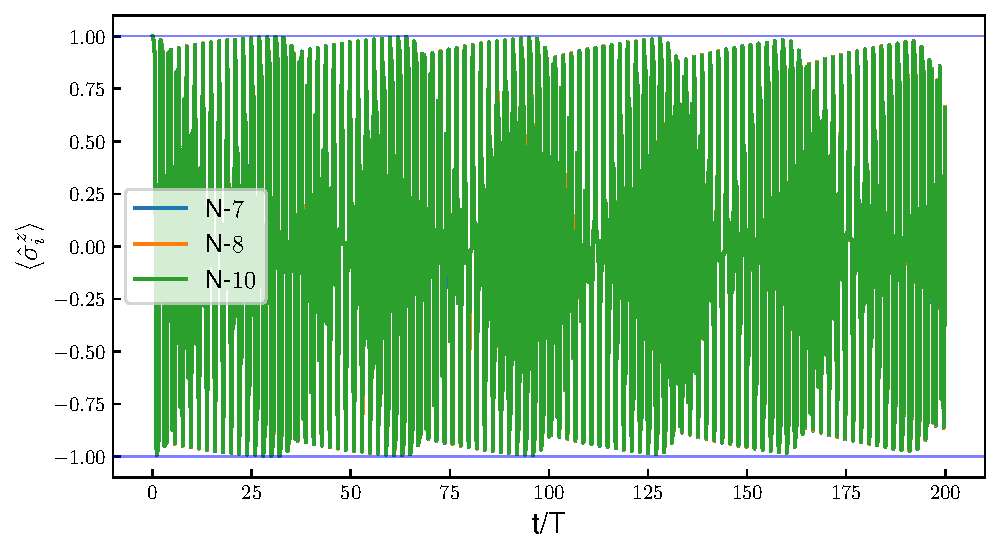
\includegraphics[width=0.45\textwidth]{figs/DTC_mag_inset_er=0.03_J=1_g=1.pdf}
    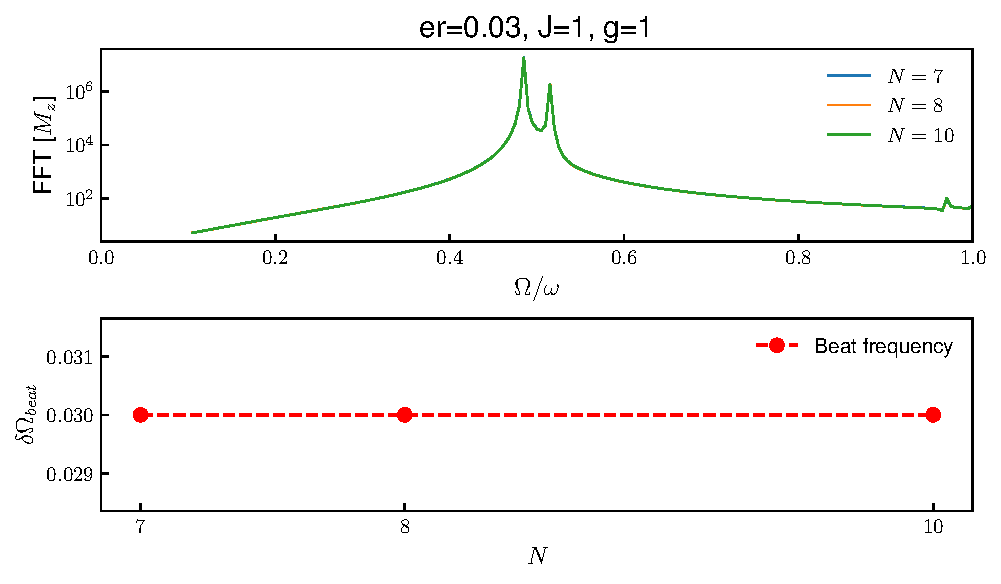
\includegraphics[width=0.45\textwidth]{figs/DTC_mag_fft_inset_er=0.03_J=1_g=1.pdf}
    \caption{Time evolution of the magnetization for a system initialized in the fully polarized state, $\ket{\psi(0)} = \ket{\uparrow \uparrow \uparrow \ldots \uparrow}$, with a small rotational error ($\epsilon = 0.03$) in the spin-flip operation. Top panels: Moderate interaction strength ($J=0.18$, $g=J/2$) shows gradual decay of period-doubled oscillations due to the impurity term. Bottom panels: Stronger interactions ($J=1$, $g=1$) result in more rapid decay and faster loss of DTC order. The right panels display the corresponding Fourier transforms, highlighting the presence of subharmonic peaks at $\omega/2$.}
    \label{figs:clean_flatband_dtc_er}
\end{figure}



\end{document}